\chapter{Introduction}
There are many tools on the internet for building graphs to visualize data. Famous examples are "ConceptDraw Pro", "Lucidchart" (https://www.pcwdld.com/top-10-network-diagram-topology-and-mapping-software) or "draw.io". However when using these the user spends a lot of time on creating a nice looking diagram, centering important components etc., to get a pleasant looking result in the end.

The idea for this project is to offer an online editor with CRUD-functionality for a network, consisting of components of software projects, as well as a first implementation of an algorithm that will, in most cases, create a nice looking layout on its own.

\section{Purpose}
The purpose is to try out and test a combination of technologies. This software, or variations of it, might later be incorporated into a bigger project or adapted to fit another use case. The experiences and impressions during development can be of help when thinking about what technology stack to use, which is why a big part of this paper is dedicated to documenting this process.

\chapter{Backend to Frontend}
In this chapter we will introduce the individual components, tools and frameworks this application is built with. For some of them we will give some more insights on how they work internally, the others are big enough on their own. The order will be the same as they appeared in the development process.

\section{The GRAND-stack}
GRAND stands in this case for \textbf{G}raphQL, \textbf{R}eact, \textbf{A}pollo and \textbf{N}eo4j \textbf{D}atabase. (https://grandstack.io/docs/getting-started-neo4j-graphql) React is a frontend framework, Apollo is used for statemanagement on the client side and communicating to the database on the server side. GraphQL will be used for fetching and mutating data. Neo4j is a graph database and the server will communicate with it through a JavaScript driver provided by the Neo4j community. More details can be found in the Development and Documentation section.

\section{Query Language - GraphQL}
GraphQL is a data query language as well as specification. Its development was started by Facebook in 2012 and it was open sourced in 2015. (https://foundation.graphql.org/)\\
After their application suffered from poor performance on mobile devices, they took a new implementation using natively implemented models and views. This required a new API for their news feed as it was previously delivered as pure HTML.\\
After evaluating different common options like RESTful-APIs and FQL they often saw the same problems:  The ratio of data actually used compared to the one fetched was very small, the number of requests (https://www.youtube.com/watch?v=zvZP0PVAdR0) and the amount of code on both server and client side to prepare the data was big. (https://engineering.fb.com/core-data/graphql-a-data-query-language/)\\
For example, for loading the start page of a single user, there would have been a lot of different requests necessary: (https://www.youtube.com/watch?v=zvZP0PVAdR0)
\begin{itemize}
\item \emph{https://facebook.com/user/id} - Get all user specific data
\item \emph{https://facebook.com/user/id/events} - Get all possibly relevant events
\item \emph{https://facebook.com/user/id/friends-suggestions} - Get all friend suggestions
\item ...
\end{itemize}

GraphQL aims to resolve all these issues: Reduce the amount of unnecessary data transferred, reduce the number of requests and increase the developer productivity by making it easier to use fetched data. (https://engineering.fb.com/core-data/graphql-a-data-query-language/)

It allows developers to get a lot of different data from a single endpoint. This means that instead the above shown 3+ endpoints, when using GraphQL all requests would go to \emph{graph.facebook.com}, with a query similar to:\\ (https://www.youtube.com/watch?v=zvZP0PVAdR0) (todo: define graphql styles)
\newpage
\begin{lstlisting}[caption={A GraphQL Query},label={ex211}]
query {
	user(id: 1) {
		name
		events {
			count
		}
		friends_suggestions {
			name
			mutual_friends {
				count
			}
		}
	}
}
\end{lstlisting}

Where the answer would be a JSON-string: (todo: define JSON style)
\begin{lstlisting}[caption={Example Response Data},label={ex212}]
{ 
	"data": {
		"user": {
			"name": "Brandon Minnick",
			"events": {
				"count": 4
			},
			"friends_suggestions": {
				"name": "Seth Juarez",
				"mutual_friends": {
					"count": 18 
				}
			}
		}
	}
}
\end{lstlisting}

The query can be as extensive as the developer needs it, it will return only the data requested and the answer string can be directly accessed like a JSON-object. By that GraphQL fulfills all its design goals.
\\ \\
The previously shown query then needs to be resolved by a server thats able to interpret GraphQL and resolve the query. All non primitive data types have to be defined following the GraphQL specification. An example for a user schema might be:

\begin{lstlisting}
type User {
	id: ID! 
	name: String! 
	events: [Event] 
	friends: [Friend] 
	friends_suggestions: [Friend_Suggestion] 
}
\end{lstlisting}

\noindent
where "Event", "Friend" and "Friend\_Suggestion" themselves are other types described in a similar manner.

By putting a "!" behind a property the programmer marks it as required, meaning it can never be null or empty. The square brackets define that the property is a list of the type they surround. (http://spec.graphql.org/June2018/)
\\
To be able to run queries in the first place, one must first define a root type for all queries:

\begin{lstlisting}
schema {
	query: Query
}
\end{lstlisting}

In this root type all possible queries must be described:

\begin{lstlisting}
type Query { 
	user(id: ID!): User 
}
\end{lstlisting}

Here we describe a query that can be executed as shown in
\textbf{\ref{ex211}} by providing an ID to the query and the correct query name, together with a collection set telling the server which fields to fetch. In the parentheses any query arguments are listed, in this example id must be provided. After the double dot the return type is named. 
\\
The server will then make requests to the DB, fetch the requested data and return it to the user once all fields were filled with values.
\\
For further information about the extensive type system please see the official GraphQL specification. (http://spec.graphql.org/June2018)

\section{Database - Neo4j}
\subsubsection{General}
Neo4j is a so called graph database. The idea of graph databases is, compared to traditional relational databases, a young concept and differs in a few concepts. At the moment Neo4j is the 22nd most popular database overall (https://db-engines.com/en/ranking) and the most popular graph database. (https://db-engines.com/en/ranking/graph+dbms)

\begin{itemize}
\item Unlike most relational databases, who store data through tables and joins, Neo4j stores data in the form of actual nodes and relationships between such (https://neo4j.com/developer/neo4j-database/). In other DBMS relations between items generally are achieved through join-/lookup-tables which have to be generated. (https://neo4j.com/developer/graph-db-vs-rdbms/)

\item When running a query on a relation DB the server will run through a table and when it finds the searched item it might look for the ID of a related item and start indexing again. With a graph DB the server will index (https://skillsmatter.com/skillscasts/2968-neo4j-internals around 32:45) once to find the initial node and can then directly access all connected items as they are stored through their relation with the current one. (https://www.youtube.com/watch?v=REVkXVxvMQE) These are stored as memory pointers which makes following them extremely efficient.
\item Neo4j uses Cypher as query language. The Cypher syntax was supposed to visually represent the shape of the data a user wants to retrieve instead of describing how to get data, as well as offer the power and functionality other languages offer. (https://neo4j.com/developer/cypher-query-language/) 
\end{itemize}

\subsubsection{Cypher}
For matching all nodes connected to node A through a "Neighbor" relationship, we simply state
\begin{exmp}
\label{ex231}
\emph{MATCH (n:Node \{label: "A"\})-[:Neighbor]-(n2:Node) RETURN n, n2 }
\end{exmp}
Parentheses represent a node, square brackets a relationship. The naming works after the following pattern: <name>:<type>. In this example n is the name for the first node and n2 the name of the list of connected nodes. We didn't specify a name for the relationship as we did not want to retrieve data from it. By using curly braces we can specify certain properties a node or relationship should have. The other way of doing so would be 
\begin{exmp}
\label{ex232}
\emph{MATCH (n:Node)-[:Neighbor]-(n2:Node) WHERE n.label = "A" RETURN n, n2 }
\end{exmp}
which might look a bit cleaner. We could also return only specific values of n and n2 and give them names by stating \\
\emph{ ...RETURN n.label AS Label1, n2.label AS Label2 }\\
The following information about Neo4j internals is all from (https://skillsmatter.com/skillscasts/2968-neo4j-internals) and (https://www.slideshare.net/thobe/an-overview-of-neo4j-internals). Sadly, these sources are all old and probably outdated, yet there does not seem to be more updated information on the internet.
\subsubsection{The Graph on Disk}
Internally, there are 3 types of records saved on the disk: node-, relationship- and property-records. All of these have fixed sizes to allow for quicker allocation during the start up process. Every record has an "inUse" field, as well as a unique ID with which Neo4j is able to exactly locate a searched record on the disk. (Video be ca. 08:27) \\
Properties on nodes are saved through a linked list like object. The exact implementation however does not alter the idea behind it. A property knows about its type and has a next pointer. Each node saves the pointer to its first property whose next pointer will lead to the next property etc.. Should a next pointer be empty the algorithm knows that it has reached all properties of a node. \\
In addition to the first property, each node knows about its first relationship. If a it is the \emph{first} one, is simply being determined by the order of creation. A relationship has pointers to its start- and end-node, to its type and four others to other relationships, which are best explained in an example traversal in pseudo code:
\begin{lstlisting}
if node n has relationship pointer r: 
	if n is start node of r: 
		if r has StartNext pointer sn: 
			set r = sn 
			repeat from line 2 
		endif 
		else  
			visited all relationships $ \rightarrow $ terminate
		endelse 
	endif 
	else 
		if r has EndNext pointer en: 
			set r = en 
			repeat from line 2 
		endif 
		else
			visited all relationships $ \rightarrow $ terminate
		endelse 
	endelse 
endif
\end{lstlisting}

\noindent
We see that every relationship has two next pointers. Which one will be used for further traversal, depends on if the source node is start- or end-node in the current relationship. \\
In addition to this, the same pointers exist into the other direction, meaning that there are also two pointers called StartPrevious and EndPrevious. The question for selecting which one will be chosen for further iteration stays the same.

\subsubsection{The Graph in Memory}
Upon start up these records are being loaded into the "FS Cache" (File System Cache). Neo4j will then partition these into equally sized regions and create a hit counter for each of them, to encounter high traffic regions that will be loaded into the "Node/Relationship Object Cache" which is more similar to an actual graph. \\
Here each node holds a list of relationships that are grouped by the relationship type to allow for quick traversals, and relationships only hold their properties as well as start- and end-node and their type. Any references to other records are being done by its ID. 

\subsubsection{Traversing}
For finding a node to start traversing the graph, Neo4j uses traditional indexing. (https://skillsmatter.com/skillscasts/2968-neo4j-internals around 32:45) Once the start node is found, 2 concepts take over:
\begin{enumerate}
\item \textbf{RelationshipExpanders} which will for a node return all relevant relationships to continue traversing from that node
\item \textbf{Evaluators} which return if traversing should continue on this branch ($ \rightarrow $ expand) or not and if this node should be included in the result set or not.
\end{enumerate}
When accessing a node the first thing the system will try to do is fetch it from the cache. If it shouldn't be there, the next place that will be checked is the FS Cache. Should the region that contains the node be apparent here, the access is quick but blocking, meaning that the entire region is getting locked. In the case that the region is out of the FS cache the operation is blocking and slower. \\
The locking is necessary to make sure that no other transaction will evict that area from the memory while the current one reads the data.

\subsubsection{Adding Cypher}
As Cypher describes the shape of the searched data, a searched query will be converted into a representative pattern graph that matches the searched structure. \\
When a query is run, the first thing that happens is that matching start-nodes are searched in the database (through indexing). When a node is found, traversing the database starts as described above. For Expanders and Evaluators to know what to return, they simply compare the pattern graph described through Cypher with the graph that was found so far and see if there is more data that matches. 

\section{Server - ApolloServer}
%maybe some general information about Apollo?
Apollo Server is a spec-compliant GraphQL server (https://www.apollographql.com/docs/apollo-server/). It can be embedded into Node.js middleware like Express or Fastify and will listen for connections on a defined port. \\
When it receives one it will read the query and call the respective route, or resolvers as they are called. \\
In addition to that the server will deliver, together with some more, a \emph{context} object to each route that contains a driver which connects to a database, which is Neo4j in our case. Using this object together with a specified Cypher query we can manipulate the DB. 

\subsubsection{Example Resolver}
A resolver to create a node might look like the following:

\begin{lstlisting}[caption={A Basic Resolver},label={ex241}]
async CreateNode( _, args, ctx ) { 
	const session = ctx.driver.session(); 
	const query = ` 
			CREATE (n:Node:${ args.nodeType } {id:$id, label:$label, nodeType: $nodeType}) 
			SET n += $props 
			RETURN n`; 
	const results = await session.run(query, args);
	return results.records.map(record => record.get('n').properties)[0]; 
}
\end{lstlisting}

Lets break down whats happening in this piece of code:
\begin{itemize}
\item Line 1 contains the function definition. "args" is an object that contains all data sent with the query from the frontend. "ctx" is the context object that contains the neo4j driver to communicate with the DB. The first argument "\_", which is a placeholder here as we do not need it, is the so called "parent" which is equal to the previous resolver in the resolver chain. (More about this later REMOVE THIS COMMENT)
\item In line 2 we acquire a session to communicate with the database. (https://neo4j.com/docs/api/javascript-driver/4.1/class/src/driver.js~Driver.html) Over this object we can send parameters that get executed right away.
\item Lines 3 to 6 define a Cypher query which is similar to the ones shown in \exref{ex231} and \exref{ex232}. 
\item In line 4 we make use of the args object and embed the nodeType directly into the query string by using template strings. This is necessary because at this position of a cypher query we can't make use of query variables the same way we do in the rest of the query. Later in that line we can see that by using \$<variableName> we can access query variables we pass along.
\item Line 5 demonstrates the usage of an object we can pass as query variable. This object can't only contain simple datatypes, but its really useful to set various values at once.
\item Finally, in line 7 we send the specified query string together with the args object (that must contain all referenced variables) to the database. By using the ES6 await keyword we make sure that code execution doesn't continue until the results are returned.
\item In the last line we iterate over the record set and retrieve any properties by the in the query specified name. Using only the first element of the array is specific to this case, as CreateNode is defined to return a single node, not an array of such.
\end{itemize}

\subsubsection{Resolver Chain}
To explain the resolver chain we will take a look at the following example GraphQL query: 
%(https://www.apollographql.com/docs/apollo-server/data/resolvers/#resolver-chains) (with adaptions)
\begin{lstlisting}[label={ex241}]
query GetBooksByLibrary {
	libraries { 
		branch 
		books { 
			title 
			author { 
				name 
			} 
		} 
	} 
}
\end{lstlisting}

which will be executed on this schema 
%(https://www.apollographql.com/docs/apollo-server/data/resolvers/#resolver-chains) (with adaptions)
\begin{lstlisting}[caption={Schema Definition},label={ex242}]
# A library has a branch and books 
type Library { 
	branch: String! 
	books: [Book!] 
} 

# A book has a title and author 
type Book { 
	title: String! 
	author: Author! 
	branch: String! 
} 

# An author has a name 
type Author { 
	name: String!
} 

type Query { 
	libraries: [Library] 
}
\end{lstlisting}

\noindent
To resolve the query we need 4 resolvers:
\begin{itemize}
\item A root resolver which defines the entry point for the query
\item One resolver each for "Library", "Book" and "Author"
\end{itemize}

\noindent
Assuming we have static arrays called "libraries", "books" and "authors" that are filled with data, the resolvers might look like the following: 
%(https://www.apollographql.com/docs/apollo-server/data/resolvers/#resolver-chains) (with adaptions)
\begin{lstlisting}[caption={Resolver Definition},label={ex243}]
const resolvers = { 
	Query: { 
		libraries() { 
			return libraries; 
		} 
	}, 
	Library: { 
		branch(parent) { 
			return parent.branch; 
		}, 
		books(parent) { 
			return books.filter(book => book.branch === parent.branch); 
		} 
	}, 
	Book: { 
		title(parent) { 
			return parent.title; 
		}, 
		author(parent) { 
			return authors.find(author => author.name === parent.author.name); 
		} 
	}, 
	Author: { 
		name(parent) { 
			return parent.name; 
		} 
	}
};
\end{lstlisting}

First, the Query resolver is hit and it will search for a defined key that is similar to the name mentioned in the highest level of the query object in \textbf{\ref{ex241}}, in this case "libraries". In the GraphQL schema under \textbf{\ref{ex242}} we defined that this query will return an array of Library objects. \\
Knowing this, the server will now go through each object of this array and look for resolvers of the in the query specified fields. This object is passed as \emph{parent} into the next resolver in the resolver chain. \\
For each library we want the branch and an array of books. As branch is a primitive type it does not need to be further resolved. Books however, returns an array of non-primitive types. To find out which books we need to return we can access the value \emph{parent.branch} and compare it to the branch of each book in the books array and return those who match. \\
books is again an array of a non primitive type and has to be further resolved by iterating through the array and accessing the requested values title and author. Title is just a string, whereas author will get resolved further etc.

\subsubsection{Cypher in GraphQL}
Using GraphQL directives we can "annotate" our schema and specify precisely certain actions or checks the server should perform when accessing a field. \\
We could create the following schema: 
%(https://www.graphql-tools.com/docs/schema-directives/#implementing-schema-directives)

\begin{lstlisting}[caption={Example Directive Declaration}]
directive @deprecated( 
	reason: String = "No longer supported" 
) on FIELD_DEFINITION | ENUM_VALUE 

type ExampleType { 
	newField: String 
	oldField: String @deprecated(reason: "Use `newField`.")
}
\end{lstlisting}

Directives can be distinguished by the @-symbol and are placed after a field definition to annotate one. When querying \emph{oldField} on \emph{ExampleType} the server might only respond with "Use 'newField'" and not send any data. The exact behavior depends on how directive behavior is defined in the server. \\
The use cases range from formatting strings, enforcing access permissions to value checking when the client sends data and many more. For information about how directives can be implemented please refer to
%(https://www.graphql-tools.com/docs/schema-directives/#implementing-schema-directives)
\\
In the GRAND-stack we can use a pre-defined directive called "@cypher" and through that use cypher statements directly in the schema definition file. A great and short example is getting all connected nodes for a specific node:

\begin{lstlisting}[caption={Cypher in GraphQL}]
type Node { 
	... 
	connectedTo: [Node] @cypher(statement: "MATCH (this)--(:Link)--(n:Node) return n") 
	...
}
\end{lstlisting}

The node that is currently being iterated over in the resolver chain is passed as \emph{this} to Neo4j. Then it'll look for other nodes that are connected through any relationship of type \emph{Link} and return these. In addition to this, ApolloServer can generate default resolvers for queries and mutations meaning we do not have to write a resolver for \emph{Node} on our own. This combination makes writing query resolvers a rare occasion when using the GRAND-stack. \\

Please note that this feature is only available when \emph{APOC} is enabled on this Neo4j instance (more information about this in the end of chapter 3 and chapter 4).

\section{Frontend - React}
React is a JavaScript-Framework to create component-based user interfaces. Each component has to define a \emph{render} method which describes what appears on the screen. In this method the programmer writes basic HTML or can embed other react components. \\
The standard \emph{index.html} is pretty short when using react. The only code a programmer writes there is normally in the header area to include CDNs or other resources. The body contains only one element: \\
\emph{<div> id="root"></div>} 

\subsubsection{Components}
In \emph{index.js} this root div will be referenced by the react-internal render method and recursively build the basic html out of the defined react components:

\begin{lstlisting}[caption={Hello World in React},label={ex251}]
// index.html:
<!DOCTYPE html>
<html>
<head>
	<title>Intro-App</title>
</head>
<body>
	<div id="root"></div>
</body>
</html>

// index.js:
ReactDOM.render(
	<App/>,
	document.getElementById( 'root' ),
);
// App.js:
import React from 'react';

class App extends React.Component {
	render() {
		return (
			<div>
				Hello World
			</div>
		);
	}
}

export default App;
\end{lstlisting}

We define a class component by extending from \emph{React.Component}. Each class component must at least have a \emph{render()} method. React will use the return values of these methods to build the DOM.

When we start the react app, open it in the browser and select inspect we will see the following in the "Elements" tab (ignoring a script for live updates in the head):

\begin{lstlisting}
<html> 
<head>
	<title>Intro-App</title>
</head>
<body>
	<div id="root">
		<div>
			Hello World!
		</div>
	</div>
</body>
</html>
\end{lstlisting}

React starts traversing at whatever component is put into the \emph{ReactDOM.render} method and repeats the process for each component until primitive html elements that can be rendered directly are reached.

Every react class components can receive values from its parent element, by passing them like normal html properties (e.g. line 3 below). In the child they can be accessed through a variable called \emph{props} and using JSX we can embed the value of variables directly in the component (e.g. line 14 below):

\begin{lstlisting}[caption={Using Props},label={ex252}]
// index.js:
ReactDOM.render(
	<App text={ 'Hello World' },
	document.getElementById( 'root' ),
);

// App.js:
import React from 'react';

class App extends React.Component {
	render() {
		return (
			<div>
				{ this.props.text }
			</div>
		);
	}
}
export default App;
\end{lstlisting}
Both \textbf{\ref{ex251}} and \textbf{\ref{ex252}} will produce the exact same output.

\subsubsection{State}
React class components have a state which can be used to manage user actions on a component, as well as general application data. \emph{state} is a simple JavaScript object but should be treated as immutable and only be updated through the \emph{setState()} method. Modifying the state directly can lead to bugs and/or unexpected behavior of the application.

To demonstrate this, we'll add a \emph{Counter} component to the application:

\begin{lstlisting}
// index.js
import React from 'react';
import ReactDOM from 'react-dom';
import App from './App';

ReactDOM.render(
	<App text={ 'Hello World' }/>,
	document.getElementById( 'root' ),
);

// App.js
class App extends React.Component {
	render() {
		return (
			<div>
				{ this.props.text }
				<Counter/>
			</div>
		);
	}
}
export default App;

// Counter.js
import React from 'react';

class Counter extends React.Component {
	constructor( props ) {
		super( props );
		this.state = { val: 0 };
		this.increase = this.increase.bind( this );
		this.decrease = this.decrease.bind( this );
	}

	increase( e ) {
		e.stopPropagation();
		let { val } = this.state;
		val++;
		this.setState( { val } );
	}

	decrease( e ) {
		e.stopPropagation();
		let { val } = this.state;
		val--;
		this.setState( { val } );
	}

	render() {
		return (
			<div>
				<p>Current score: { this.state.val }</p>
				<button onClick={ this.increase }>+</button>
				<button onClick={ this.decrease }>-</button>
			</div>
		);
	}
}
export default Counter;
\end{lstlisting}

When defining a custom constructor for a class component it is necessary to call \emph{super( props )} first. To define an initial state of the component we can set \emph{this.state = \{ val: 0 \}}. This is the only place where state should modified directly. In comparison to that in lines 43 and 50 we first create a copy of the value we want to modify by using Object Destructuring and then use \emph{this.setState( \{ val \} )} to update it. By doing so we do not modify the state object directly.

In lines 31 and 32 we bind the this keyword on the increase and decrease functions. By leaving this step, accessing \emph{this.setState()} in any of the methods would crash the application as \emph{this} would be the global window object which doesn't have a \emph{setState} method defined.

The render method defines the output of the component. We'll render a paragraph telling the current score by accessing the state together with two buttons and their respective click handlers.

\subsubsection{Updating Components}
React is known for its good performance (https://dev.to/spukas/react-work-phases-4eaj) even in large applications. To understand better how it achieves this, we will look a bit at the internal process of rendering and updating the components.

On the initial render React will create a component tree from which it'll then build the DOM that the browser converts into displayable objects and paints them on the screen. To show how react determines which part of the DOM it has to update, we'll quickly walk through the previous example:

When clicking the increase or decrease button in the previous example we update the components state which will automatically trigger a re-render. In such a small component it wouldn't really matter if React simply rendered the whole component. In a component containing hundreds of lines and probably many other sub-components the decision to render all of just because, would take a long time and be fatal for performance especially if really all we'd have to do is re-render line 52.

\subsubsection{Finding The Differences} (maybe when coming back to this check https://reactjs.org/docs/faq-internals.html https://reactjs.org/docs/reconciliation.html and https://github.com/acdlite/react-fiber-architecture  and THIS:: https://www.youtube.com/watch?v=RquK3TImY9U )
To know which lines to update, React performs a few steps: 
\begin{itemize}
\item The \emph{setState} function will mark the component and all its children as dirty. (https://medium.com/@gethylgeorge/how-virtual-dom-and-diffing-works-in-react-6fc805f9f84e großes Bild)
\item It'll recursively walk through all components marked as dirty, building them in the virtual DOM
\item For each built element it compares it to the value in the actual DOM. If they differ it'll deduce if the item should be replaced, removed or updated and does so accordingly. 
%https://overreacted.io/react-as-a-ui-runtime/#reconciliation
\end{itemize}
By doing so, instead of re-rendering the whole \emph{Counter} component it only re-renders
\begin{lstlisting}
<p>Current score: { this.state.val } </p>
\end{lstlisting}

\subsubsection{Stateless Functional Components}
It is also possible to create stateless functional components. In their pure form they do not contain state and normally only show either static data or data they get passed through props. If we look at the \emph{App} component in the above examples we'll find that it does exactly that. Knowing this, we could re-write it:
\begin{lstlisting}
// App.js
import React from 'react';
import Counter from './Counter';

function App( props ) {
	return (
		<div>
			{ props.text }
			<Counter/>
		</div>
	);
}
export default App;
\end{lstlisting}
Which is a lot shorter and has another big advantage: It protects from laziness. (https://hackernoon.com/react-stateless-functional-components-nine-wins-you-might-have-overlooked-997b0d933dbc) As this component doesn't support local state it is not too tempting to quickly hack something new into it. Rather the programmer gets encouraged to think about the structure and create a proper component for a new feature together with its own state object that only that component needs.

And of course visually the result is equal to the one in \textbf{\ref{ex251}} and \textbf{\ref{ex252}}.

\section{Client - ApolloClient}
ApolloClient is a state management library for JavaScript that manages data with GraphQL. It offers an all in one solution for fetching, caching and modifying application data and together with automatic UI updates upon events from the server. (https://www.apollographql.com/docs/react/)

\subsubsection{Hooks}
ApolloClient 3 offers this by providing custom \textbf{hooks}. Hooks are a new addition to React since React 16.8 and were introduced to improve stateless functional components (https://reactjs.org/docs/hooks-intro.html) and can only be used in such (https://reactjs.org/docs/hooks-overview.html). There were a few reasons that led to the introduction of hooks like the appearance of complex class components that couldn't be split into smaller ones, not re-usable stateful logic and classes being not ideal for future optimization. (https://reactjs.org/docs/hooks-intro.html) Hooks allow for example the usage of state in functional components.

\subsubsection{Apollo Hooks}
In addition to some built-in Hooks provided by React it is also possible to create them. Apollo implemented many own hooks, we will focus on \emph{useQuery}, \emph{useLazyQuery} and \emph{useMutation}.
The first argument to all of these is a GraphQL string. A query for the first two, a mutation for the last one.

The second argument is the options object. By adding properties to this the execution behavior can be influenced. Probably the most important argument is \emph{variables}. This is an object containing key-pair values that equal to the ones used in a GraphQL query as shown in \textbf{\ref{ex211}}. In addition to that there are \emph{onError} and \emph{onCompleted}. These are two callback functions that allow for executing actions upon completion or handling of possible errors. Imagine \emph{GET\_DATA} being a valid GraphQL query string:
\begin{lstlisting}
function Test() {
	useQuery( GET_DATA, {
		variables: { id: 1 },
		onCompleted: data => console.log( data );
		onError: error => console.log( error.message );
	} );
	...
}
\end{lstlisting}

For the rest of the arguments please refer to (https://www.apollographql.com/docs/react/api/react/hooks/)

To be able to use returned data and inform the user about the current status, all of these three hooks return a few other objects, the most important being \emph{data}, \emph{loading} and \emph{error}. These are boolean values and allow for conditional rendering inside a component, depending on their values: 
\begin{lstlisting}
function Test() {
	const { data, loading, error } = useQuery( GET_DATA, {
		...	
	} );
	
	if ( loading ) return 'Fetching data.';
	if ( error ) return 'Error when fetching data.';
	return 'Success!';
}
\end{lstlisting}

In comparison to \emph{useQuery} the other two also return a function object that can be called when we wish to execute the query or mutation (see example below).

The \emph{useMutation} hook is the only one of the three allowing for an \emph{update} argument in the options object. In this we can access the local cache and have access to the results returned from the mutation. This can be useful if we need to update internal data depending on the result of a server operation:
\begin{lstlisting}[caption={Creating a Mutation}]
function Mutate() {
	const [ runMutation, { data, loading, error } ] = useMutation( DO_THING, {
		update: ( cache, { data } ) => {
			// update cache with return data from mutation
		}	
	} );
}
\end{lstlisting}
This approach works well and is more or less the only way of handling return results from external mutations. 

\subsubsection{Local Resolvers}
We could do the same for local state changes, but as these functions can become long it might clutter the component with a lot of code that is not actually for it. To get rid of this problem we can define local resolvers in the client instance:
\begin{lstlisting}[caption={Local Resolvers},label={ex253}]
const client = new ApolloClient({
	...,
	resolvers: {
		Mutation: {
			setData: ( _, variables, { cache } ) => {
				// manage state update			
			},
			...		
		},	
	},
	...,
});
\end{lstlisting}

Just like on the server side we set up resolvers and can access query variables to it. To call it, we also define a GraphQL query like so:
\begin{lstlisting}
const SET_DATA = gql`
	mutation SetData($data: [String]!) {
		setData(data: $data) @client	
	}
`;
\end{lstlisting}
The name in line 3 has to match with the one defined in the resolver in \textbf{\ref{ex253}} in line 5. But whats even more important is the \emph{@client} directive in the end of line 3. This tells Apollo to not contact the server, but rather resolve the mutation locally. We can then call the above defined mutation like this:
\begin{lstlisting}
const Test() {
	const [ runSetData ] = useMutation( SET_DATA );
	
	const handleClick = e => {
		e.stopPropagation();
		runSetData(	{ variables: { x: 'test' } } );
	}
	
	return (
		<button onClick={ handleClick }>Click me</button>
	);
}
\end{lstlisting}

\subsubsection{The Apollo Cache}
A unique feature of Apollo is its smart cache. Once a query to the server has been executed, the results are saved in the cache and should the exact same query be executed again, the cache will first check if it has results for this query saved locally. If so, it'll return them from there, reducing network traffic and improving performance of the whole application. 

Of course in some cases it might be necessary to always have the newest data from the cache. The exact behavior can be specified through the \emph{options} object passed to a query or mutation.
\\

The setup time for working with Apollo Client is very short as it offers great default settings that will get any application going quickly. We just looked at the absolute basics of it, it offers features like pagination, subscriptions, optimistic UI and much more.
Further it allows the programmer to define all its behavior precisely when he wants to and by that its a great tool to work with.

\chapter{Deployment}
While developing in a local environment it is also important to test the application in a production environment as early as possible. Many frameworks make optimizations to improve performance. This might lead to errors that can't be seen in a local setup. Often they also change error behavior. While during development an error might only lead to a warning message, in production the same error might cause the application to crash.

Another reason to go for early deployment is to allow other people to see, use and test the application. Someone who sees the app for the first time or at least doesn't know how things were thought to work will make completely different use of it than a programmer. New issues with the workflow can be discovered and problems that a developer would never have thought of be reported. Further the layout will be tested on different screens, browsers and devices, unveiling unknown layout troubles. Issues discovered early are much easier to fix than those who are integrated deeply into the codebase. \\

In this chapter we will talk about the tools that were used to deploy the application to a publicly available domain.

\section{AWS}
AWS is a cloud platform from Amazon that offers over 175 different services in 24 different geographic regions around the world to allow for high availability all around the world. (https://aws.amazon.com/what-is-aws/) \\
AWS was launched in 2002 only offering SOAP (a messaging protocol used in distributed systems to exchange information) and XML interfaces. (https://mediatemple.net/blog/cloud-hosting/brief-history-aws/) In 2003 the idea of a big system offering services and tools was born as the leadership realized that one of the company's strengths was building and running effective, reliable and scalable data centers. (https://techcrunch.com/2016/07/02/andy-jassys-brief-history-of-the-genesis-of-aws/) After developing a more precise idea of how this strengths could be used to fulfill a lot of companies' needs the first public launch was in 2006 with \emph{Simple Storage Service} (S3), the \emph{Elastic Compute Cloud} (EC2) and a \emph{Simple Queue Service} (SQS) following shortly after. 
%(https://mediatemple.net/blog/cloud-hosting/brief-history-aws/)

Since then the services offered by AWS keep growing and other companies like Google, Microsoft or IBM started to compete in the business. In a 2019 research from Gartner AWS was found as one of the leading cloud Infrastructure as a Service providers world wide (IaaS) 
%(https://www.gartner.com/doc/reprints?id=1-1CMAPXNO&ct=190709&st=sb) 
regarding \emph{Completeness of Vision} and \emph{Ability to execute}. 

\subsection{AWS-EC2}
EC2 is a service that allows the creation of virtual machines with over 300 different variations of computational capacities like the number of CPUs, Memory, Storage and Network Performance.
%(https://aws.amazon.com/ec2/?nc1=h_ls) 
Available configurations that can run on an instance are called Amazon Machine Images (AMIs) and include various Linux based distributions like Ubuntu, Debian or fedora as well as Windows. In addition to empty operating systems Amazon and different communities also provides images with certain pre-installed software making sure that instances can be set up quickly. \\
Basically, an EC2 instance is a virtual machine that runs on an Amazon server. (https://www.quora.com/Is-EC2-a-virtual-machine)

%In this app we will make use of EC2 to run a Neo4j instance. To make configuration easier, the Neo4j community provides images that can be started directly with only a few clicks from the AWS EC2 management console. By selecting AMIs and searching for "neo4j-community" in public images we can see all the available images with different versions of Neo4j. We will select one of the images that contains \emph{apoc} in their name to be able to use Cypher in our GraphQL schema. After clicking Launch we can select an instance https://neo4j.com/developer/neo4j-cloud-aws-ec2-ami/

\subsection{AWS-ECS}
ECS is a service to run automatically managed containers on AWS servers. Many big companies make use of this service because of its scalability, reliability and security. 
%(https://aws.amazon.com/ecs/?nc1=h_ls)
These are the most important terms when talking about AWS ECS: \\

A \textbf{definition} is the blueprint of a task, specifying which Docker image(s) to use, ports to expose, can set environment variables and memory needed etc. (https://www.freecodecamp.org/news/amazon-ecs-terms-and-architecture-807d8c4960fd/)

A \textbf{task} is an instance that is created following the specifications in the task definition. A task can run various Docker containers at once. A task is where an application actually gets executed.

A \textbf{service} is used to manage tasks. It is possible to specify a minimum and maximum number of running tasks and when to start new or stop running tasks to make sure the necessary calculation power is always necessary. A service can make use of a load balancer which will distribute network traffic equally over all running tasks in the service.

A \textbf{Cluster} is a logical grouping of services. \\

<<<<<<< HEAD
These components can be visually put together as shown in figure \textbf{\ref{ex311}}. (https://docs.aws.amazon.com/AmazonECS/latest/developerguide/Welcome.html)
=======
These components can be visually put together as shown in the figure below. (https://docs.aws.amazon.com/AmazonECS/latest/developerguide/Welcome.html)
>>>>>>> 4d6893b6d823151844e816054fcf2ceb16956cf6
\begin{figure}[H]
\centering
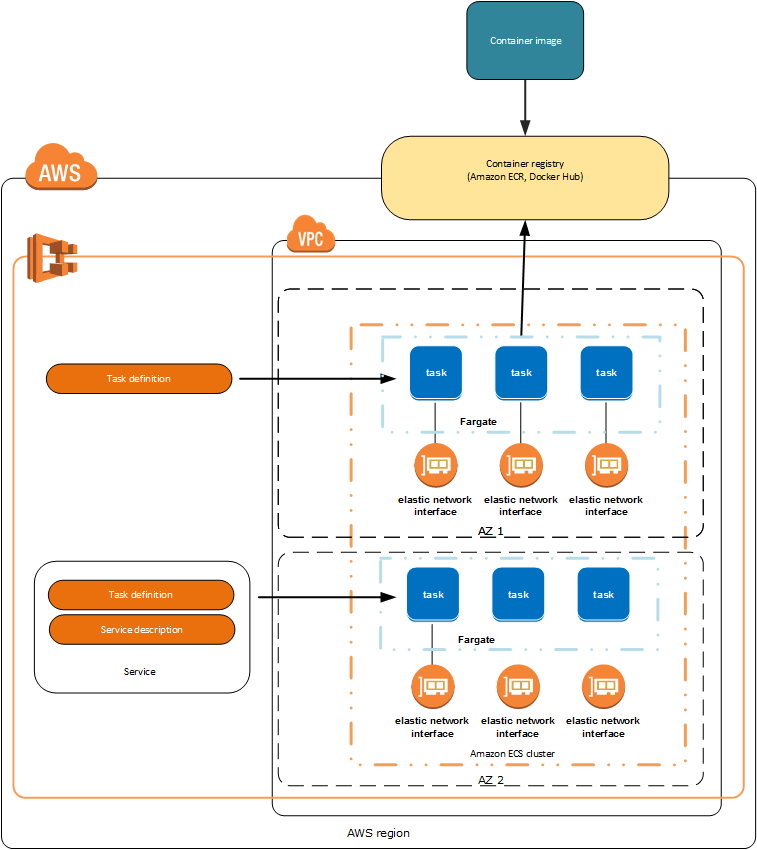
\includegraphics[scale=.85]{Bilder/overview-fargate.png}
\captionof{figure}{Strucute of AWS ECS}
\label{ex311}
\end{figure}

The orange square symbolizes ECS inside the big AWS infrastructure. We will ignore the square denoted with "VPC" as it is not relevant for further understanding.\\
A task can be created from a task definition and be placed in a service. The services are here shown as light blue squares labeled \emph{Fargate}. Fargate is a computation engine from Amazon which calculates which virtual machine to use according to the task definition and creates and starts it and then runs the docker image from a specified container registry automatically. (https://aws.amazon.com/fargate/) The orange square with dots and dashes is a cluster. This cluster contains 2 services, reach running 3 tasks. 

The services of a cluster can be run in different \emph{Availability Zones} (AZ), meaning that they run on servers from AWS located in different parts of a geological region.

\subsection{AWS-Amplify}
Amplify is a services that aims to make the deployment as well as the development of applications as easy as possible. It comes with many advanced features that help setting up an app quickly. Some examples are: Authentication, API creation, Analytics, Push Notifications and many more (https://aws.amazon.com/amplify/). It creates a certificate for any deployed application, allowing for HTTPS connections. Further it is able to scan a connected GitHub repository and provide a template configuration based on the framework used.

Another really nice feature is the easy deployment flow: For each application it is possible to connect various branches. Each branch will have its unique URL and once a developer pushes to a connected branch, Amplify will build the newest status of the application. This is a great feature for testing new features in a production environment without having to deploy to a master server directly.

\section{Docker}
Docker is a platform that provides the ability to a developer to create any environment in which he wants to execute code in.
Before comparing it to a virtual machine we'll take a look at the basic terminology:

A \emph{Docker File} is a text file containing instructions that tell the Docker Engine how to build a \emph{Docker Image}. (https://nickjanetakis.com/blog/differences-between-a-dockerfile-docker-image-and-docker-container)

This \emph{Docker Image} is a file containing necessary data to execute a given program. The in the docker file specified libraries are saved, folders from the local machine are copied, environment variables are set etc.. 

When running the image, we will get a \emph{Docker Container}. It will execute specified commands and by that for example download node modules. This container is an instance executed by the \emph{Docker Engine} which runs on top of the Host OS of an actual machine.
\\

While it is similar to a virtual machine, there are certain differences between them: (https://geekflare.com/docker-vs-virtual-machine/)\\
\textbf{Operating System} Every VM comes with its own operating system, making it heavy in terms of memory and processing power they require. Docker containers in turn all share the hosts operating system and only require the docker engine to be installed on the machine: (inspired by https://geekflare.com/docker-vs-virtual-machine/)
\begin{figure}[H]
\centering
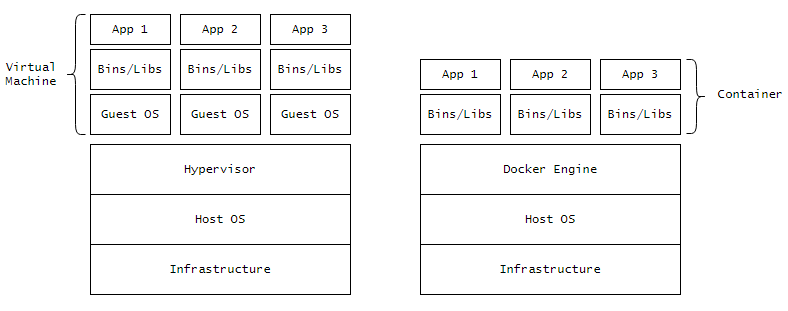
\includegraphics[scale=.8]{Bilder/DockerVsVM.png}
\captionof{figure}{Docker vs VM}
\label{ex312}
\end{figure}
\noindent
\textbf{Security} Following the previous point, every VM has its own operating system and is strongly isolated in the host kernel. Docker containers all run on a single kernel. Furthermore docker resources are shared. If an attacker gets access to one container he'll be able to exploit  all containers in a cluster. (https://geekflare.com/docker-vs-virtual-machine/) \\
\textbf{Portability} Containers can easily be ported to any machine that has the docker engine installed. There is no further configuration necessary, they'll the same on any machine. VMs are more difficult to port just due to their sheer size. In addition, the process of setting up a virtual machine differs from operating system to operating system. 

\chapter{Development}
\section{Getting started with Neo4j}
\section{Manipulating the DB through ApolloServer and GraphQL-Playground}
\section{Making ApolloServer and ApolloClient communicate through GraphQL}
\section{Building the UI}
\subsection{Components}
\section{Problems}
\subsection{Keeping the data consistent when saving changes}
\subsection{AWS-Healthcheck}
\subsection{Apollo Error-Codes}
\subsection{Apollo Chrome Dev-Tools}
\subsection{Graph-Layout}
\subsubsection{Tree-Layout}
\subsubsection{Flower-Layout}
\section{Behavior Decisions}
\section{Avoiding data corruption through multiple editors at once}
\section{Detect multiple connections between two nodes}
\section{CORS-problems}

\chapter{Looking back}

\chapter{Documentation}

\chapter{Ideas for the Future}
